\chapter{Simulations}\label{c:simulations}

% In this chapter we present three different simulations. Two of which have an accompaning experimental data for micro tensile loading in the $[1\, 0\, 0]$ and $[1\, 1\, 0]$ directions of a single crystal Zn micropillar provided by Alan Xu from ANSTO Sidney. The third is is a proof of concept for a techinque developed by Jicheng Gong to cyclicly load a cantilever in opposing directions. However, this technique was developed on Ti microcantilevers and the HCP mobility law requires some adaptation before it is ready for general use. Instead we use the BCC law developed in-house by Bruce Bromage that as mentioned in the footnotes of \cref{ss:matrix}.

\section{Nickel tensile micropillar}\label{s:nickelTensile}

10 dislocations per square micron.

Square cross-section.
\subsection{Introduction}
\subsection{Methodology}

We define surface node sets $\left\{\forall (x, y, z) \in [0,\, 1] \vert S_{xyz} \in \partial \hat{V}\right\}$, where $\hat{V}$ is a unit volume such that $S_{000}$ denotes the node at the origin, $S_{x00}$ the $x$-axis spanning edge at $y,\, z=0$, and $S_{xy0}$ the $xy$-plane at $z=0$. We use these node sets to define our neuman (displacement) boundary conditions as follows.
\begin{subequations}
    \begin{align}
        S_{0yz},\, S_{0y0},\, S_{0y1},\, S_{00z},\, S_{01z},\, S_{000},\, S_{001},\, S_{010},\, S_{011} & \gets u_x = 0           \\
        S_{01z},\, S_{010},\, S_{011}                                                                   & \gets u_y = 0           \\
        S_{0y0},\, S_{010},\, S_{000}                                                                   & \gets u_z = 0           \\
        S_{1yz},\, S_{1y0},\, S_{1y1},\, S_{10z},\, S_{11z},\, S_{100},\, S_{101},\, S_{110},\, S_{111} & \gets u_x = U \neq 0\,.
    \end{align}
\end{subequations}
In simple terms, the whole $yz$-plane at $x=0$ (including corner nodes and edges) is fixed in $x$; the whole $y$-edge at $x,\,z=0$ (including corner nodes) is also fixed in $z$; the whole $z$-edge at $x = 0\,\, y = 1$ (including corner nodes) is fixed in $y$; and the nodes at $x=1$ have a displacement $U$ applied in the $x$-direction. All other degrees of freedom are free to move as necessary. Once mapped to our simulated cuboid geometry, it looks like \cref{f:tensileSetup}.
\begin{figure}
    \centering
    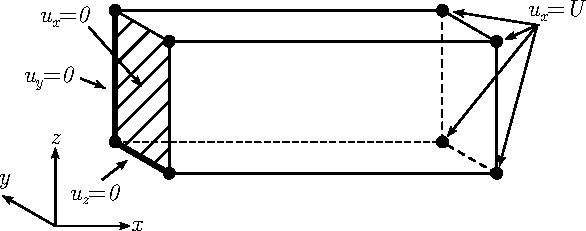
\includegraphics[width=0.8\linewidth]{tensileSetup.pdf}
    \caption[Displacement boundary conditions for dislocation plasticity modelling of single crystal, micro-tensile tests.]{Displacement boundary conditions for dislocation plasticity modelling of single crystal, micro-tensile tests.}
    \label{f:tensileSetup}
\end{figure}

In EasyDD, time is defined in units of shear modulus \cref{eq:timeConversion},
\begin{align}\label{eq:timeConversion}
    t_{\rvar{real}} & = t_{\rvar{sim}} \dfrac{B}{\lVert\mu\rVert}\,,
\end{align}
where $B \coloneqq 1 \times 10^{-4}[\si{\pascal}][\si{\second}]$ is the dislocation mobility and $\lVert\mu\rVert \coloneqq [\si{\pascal}]$ is the magnitude of the shear modulus (the shear modulus we use for the simulations is normalised to 1, its magnitude is used to scale parameters). The dislocation mobilities are normalised such that edge dislocations have mobility 1, other mobilities are defined from these. So the time conversion to real time is a matter of dividing the simulation time by the shear modulus.

The experimental loading rate provided was \SI{5}{\nano\metre/\second}, which when converted to simulation time, gives a loading rate that is far too low for the timescales we can model. So we defined $\Delta t_0 \equiv 5\times 10^{-9} \lVert\mu\rVert$ and found the maximum loading rate of the form $\dot{u} \equiv a \dfrac{\Delta l}{\Delta t_0}$, for which the quasi-static condition held true, where $\Delta l$ is the length of the beam in the loading direction and $a$ is a constant.

% size effects, microns

% 1
% 2
% 4
% 6
% 8
% 10

% dislocation density effects

% Current best loading rate for size effect
% % timeUnit = mumag * 1e6;
% % u\_dot = 1000*dx / timeUnit;

% timeUnit = 5e-3 * mumag * 1e6;
% u\_dot = 10*dx / timeUnit;

% try to push it as high as it can go without going wonky.
\subsection{Results and discussion}
\subsection{Conclusions}

\section{Tungsten cyclic loading and unloading cantilever}\label{s:tungstenCyclic}
\subsection{Introduction}
\subsection{Methodology}
\subsection{Results and discussion}
\subsection{Conclusions}

% 310


% TODO